\section{Procedure}
\label{sec:procedure}
In the following section an overview about the optical instruments is given. The important parts are
\begin{itemize}
  \item A laser as a source for coherent light (Part 2),
  \item The beam collimator (Part 4),
  \item a biconvex lens (Part 5),
  \item the Nd:YAG chrystal with mirroring coating (Part 6),
  \item a resonator mirror (Part 7),
\end{itemize}
For easier operation and measurements, a target (Part 9) and filter unit (Part 8) are used as well. 
In \autoref{fig:setup} the arrangement of the optical parts is shown, the mentioned numbers
correspond to what has been used in the manual and the figure thereof \cite{elas_manual}.
\begin{figure}
    \centering
    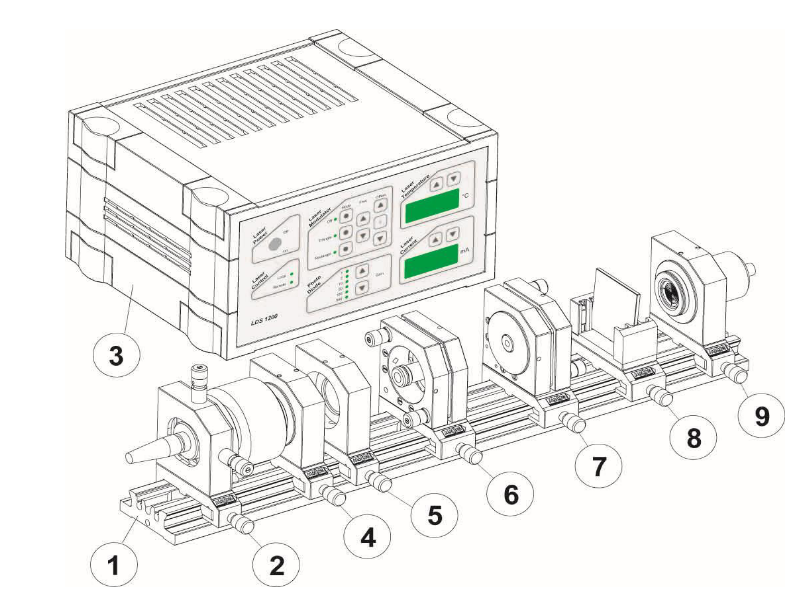
\includegraphics[width=0.4\textwidth]{media/Setup.png}
    \caption{Setup and Components of the experiment \cite{elas_manual}.}
    \label{fig:setup}
\end{figure}
The parts not mentioned yet are the power supply (Part 3) and the mounting rail (Part 1).

